\section{Economic Order Quantity}
\label{sec:deterministic}

\Opensolutionfile{ans}

% \textit{Recommended reading:} FP Section 2.2 and 2.3 covers the basic deterministic inventory models that will be considered here. We suggest you to be familiar with that material. 

In this section we study the \recall{Economic Order Quantity} (\recall{EOQ}) model, which is more or less the simplest possible inventory model. In this model we initially make a number of  assumptions: In later (sub)sections we will relax and/or change these assumptions.

\begin{itemize}
\item We are concerned with a single product inventory system.
\item Demand is constant and deterministic.
\item Stock-outs.are not allowed.
\item Lead time $L=0$.
\item Our supplier can deliver any amount of items necessary to replenish the inventory, hence is uncapacitated,  and is reliable, i.e., always deliver precisely the ordered amount precisely in time. . 
\item Items are not perishable.
\item There is a fixed ordering cost $A$ independent of the size of the order.
\item There is a procurement cost $c$ per item.
\item There is a cost $h$ per item per unit time associated with holding inventory.
\item There is no substitution effect with other item types.
\item There is no budget or storage space limitation.
\end{itemize}

The objective is to minimize long run average costs per unit time. 

\begin{exercise}
  What is the cost of placing an order of size $Q$?
  \begin{solution}
 There is a fixed cost $A$ associated with placing an order and a procurement cost $c$  per item. Thus,  the cost to get $Q$ is given by $A+c Q$.
  \end{solution}
\end{exercise}


\begin{exercise}
In reality,  demand is never known in advance. What is then the use of such deterministic inventory models?

\begin{solution}
Indeed almost all inventory management environments demand is not known in advance. But there are many cases where the variability of the demand is so low that the influence of the demand uncertainty can be safely ignored. Also, it is not uncommon to have `advance demand information' in some industries where customers place their order before they actually want it to be delivered. If this is the case, then one can  assume that the demand is known with considerable certainty over some interval of time. 

From a theoretical point of view, these models can be used as points of reference while helping you to better understanding certain trade-offs. The EOQ model has very restrictive assumptions with respect to demand, yet it is one of the most well-known models among both academics and practitioners. Finally, deterministic models --- to a certain extent --= can be adapted to account for stochastic demands and used as heuristic approaches. We will see many examples of this in this course.  
\end{solution}
\end{exercise}

% \begin{exercise}
% nvf: I dont understand this question
% The assumption of deterministic demands sounds like simplifying assumption in modeling inventories. What are it's implications?


% \begin{solution}
% Obviously knowing the demand make an inventory manager's life much easier. The main implication is simple: when you take an action, say place a replenishment order, you know exactly how this will affect the system in the future. Probably the most important result of this is that the optimal answers to the fundamental inventory control questions will not change over time as a response to realized demands. 
% \end{solution}
% \end{exercise}


The EOQ policy is very simple. When the inventory position $\IP_{i-1}$ at the end of period $i-1$ becomes equal to $0$, we place an order of $Q_i=Q$, where $Q$ is a fixed order size, i.e., 
\begin{subequations}
\begin{align}
  Q_{i} &= Q\1{\IP_{i-1}\leq 0}.
\end{align}
\end{subequations}
The dynamics follow now right away from~\eqref{eq:21}. 


\begin{exercise}
  Just to check, what is the control parameter for this model? 
  \begin{solution}
 We can only \emph{control} $Q$. Once we have fixed $Q$ to 10 say, the equations~\eqref{eq:8} determine how the inventory position behaves over time. 
  \end{solution}
\end{exercise}

\begin{exercise}
Since the replenishment lead $L=0$ for this model, how do $\IL_i$ and $\IP_i$ relate?
\begin{solution}
  $\IP_i = \IL_i \iff L=0$.
\end{solution}
\end{exercise}

\begin{exercise}
  Why is the duration of a \recall{replenishment cycle}, i.e,. the time between two order moments, equal to $Q/D$?
  \begin{solution}
    The demand is $D$ per period. After $n$ periods, the total demand is $nD$. Thus, when $n=Q/D$, the total demand is $n D = Q/D \cdot D = Q$, i.e., after this amount of time, then entire order quantity has been consumed, and we need to place a new replenishment order of size $Q$. 
  \end{solution}
\end{exercise}

\begin{exercise}
  If $Q=5$, $D=1$, and $\IP_0=0$, what are $\IP_1$, $\IP_2$, and so on?
  \begin{solution}
    \begin{align*}
      Q_1 &= Q \1{\IP_{0}\leq 0} = \1{0 \leq 0} = Q\cdot 1, \\
      \IP_1 &= \IP_0 + Q_1 - D_1 = 0 + Q - 1 = Q-1 \\
      Q_2 &= Q \1{\IP_{1}\leq 0} = \1{Q - 1 \leq 0} = 0, \\
      \IP_2 &= \IP_1 + Q_2 - D_2 = Q-1 + 0 - 1 = Q-2, \\
    \end{align*}
and so on. Since $Q=5$, $\IP_5=0$, and then the replenishment cycle starts again.
  \end{solution}
\end{exercise}

\begin{exercise}
  Explain that the total cost for a simulation of $n$ periods is equal to
  \begin{equation}\label{eq:eoq1}
    c n D + h \sum_{i=1}^n I_i + A\frac{n}{Q/D}.
  \end{equation}
  \begin{solution}
    We need to buy $n D$ items, as this is the total demand. The second term is the total cost of on-hand inventory. For the third, observe that we place orders every $Q/D$ number of periods. Thus, the total number of orders placed is $n/(Q/D)$. 
  \end{solution}
\end{exercise}

Since we have to pay the procurement costs $c$ per item anyway, and this is not affected by the control parameter $Q$, we leave it out the remainder of the computations.

\begin{exercise}
  Implement Eq.~\eqref{eq:8} and~\eqref{eq:eoq1} in excel and see how the costs are affected as a function of the order size $Q$. For instance, take $h=1$, $A=50$, $D=1$, $n=1000$, and $Q\in\{1, 2, 10\}$.
  \begin{solution}
For instance, if $Q=10$, and noting that $\IP=\IL$ since $L=0$, 
\begin{pyconsole}[eoq]
import numpy as np

D = 1
h = 1
A = 50
n = 1000

Q = 10      
IP = np.zeros(n)
for i in range(1,n):
   Qi = Q*(IP[i-1] <= 0)
   IP[i] = IP[i-1] + Qi - D

inv_cost = h*IP.sum()
inv_cost
order_cost = A*n/(Q/D)
order_cost

inv_cost + order_cost
\end{pyconsole}

What if $Q=2$?
\begin{pyconsole}[eoq]
Q = 2
IP = np.zeros(n)
for i in range(1,n):
   Qi = Q*(IP[i-1] <= 0)
   IP[i] = IP[i-1] + Qi - D

inv_cost = h*IP.sum()
inv_cost
order_cost = A*n/(Q/D)
order_cost

inv_cost + order_cost
\end{pyconsole}

As we expected, for $Q=2$, the inventory cost is  lower, but the ordering cost is much higher. 
  \end{solution}
\end{exercise}

\begin{exercise}
  Show that the average inventory level during one cycle is equal to 
  \begin{equation*}
    \frac{Q^2}{2D} - \frac{Q}2.
  \end{equation*}
  \begin{solution}
Lets focus on one cycle (all cycles being the same\ldots). Clearly, for $i\leq Q/D$, 
 $\IL_i = Q-iD$. Thus, taking $n=Q/D$, 
 \begin{align*}
   \sum_{i=1}^n (Q-iD) 
&= n Q - \sum_{i=1}^n i D = n Q - D n \frac{n+1}2 \\
&= \frac{Q^2} D - D \frac Q D \frac 1 2 \left(\frac Q D + 1\right) & \text{as } n = Q/D \\
&= \frac{Q^2} D - \frac Q 2 \left(\frac Q D + 1\right)\\
&= \frac{Q^2} D - \frac{Q^2}{2D} - \frac Q 2\\
&= \frac{Q^2}{2D}- \frac Q 2.
 \end{align*}
  \end{solution}
\end{exercise}

\begin{exercise}
If $h$ is the cost per item on hand per period,   explain that the total cost of one cycle is 
\begin{equation*}
  A + h\left(\frac{Q^2}{2D} - \frac{Q}2\right).
\end{equation*}
Just add the cost of ordering $A$ to the inventory cost, which is $h$ times the average on-hand inventory. 
\end{exercise}


\begin{exercise}
  Finally, explain that the averge cost per unit time is
\begin{equation*}
 \frac{A D} {Q}  + h\frac{Q}{2} - h\frac{D}2.
\end{equation*}
\end{exercise}

\subsection{Analysis}
\label{sec:analysis}

For the simulation of the inventory system we use discrete time and consider, for instance, the inventory level at the end of each period. For the analysis below it is slightly easier to consider that the model is under \recall{continuous-review}, that is, at each moment in time we know the system variables such that the inventory position. Here, as long as the leadtime $L=0$, we treat the inventory position and the inventory level on the same basis. 

\begin{exercise}\label{ex:2}
Sketch how the inventory position behaves over time under the EOQ policy. Explain in the graph the meaning of a \recall{replenishment cycle}.
  \begin{solution}
\begin{center}
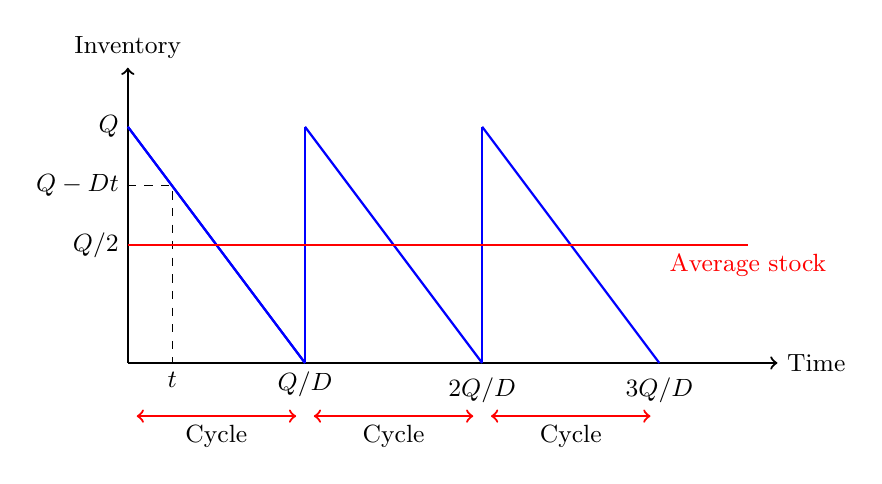
\begin{tikzpicture}[x=0.75cm,y=0.015cm]
\small
\draw[thick,->] (0,0) -- (11,0) node[right] {Time};
\draw[thick,->] (0,0) -- (0,250) node[above] {Inventory};
\draw[] (0,200) node[left] {$Q$};
\draw[color=blue,thick] (0,200) -- (3,0);
\draw[] (0.75,0) node[below] {$t$};
\draw[] (0,150) node[left] {$Q-Dt$};
\draw[dashed] (0,150) -- (0.75,150) -- (0.75,0);
\draw[] (3,0) node[below] {$Q / D$};
\foreach \y in {1,...,3}{
	\draw[color=blue,thick] (3*\y-3,200) -- (3*\y,0);}
\foreach \y in {1,2}{
	\draw[color=blue,thick] (3*\y,0) -- (3*\y,200);}
\foreach \y in {2,3}{
	\draw[] (3*\y,-5) node[below] {\y $Q/D$};}
\draw[] (0,100) node[left] {$Q / 2$};
\draw[color=red,thick] (0,100) -- (10.5,100) node[below] {Average stock};
\foreach \y in {0,...,2}{
	\draw[color=red,thick,<->] (3*\y+0.15,-45) -- (3*\y+3-0.15,-45);
	\draw[] (3*\y+1.5,-45) node[below] {Cycle};}
\end{tikzpicture}
\end{center}

  \end{solution}
\end{exercise}


\begin{exercise}
Use the graph of Exercise~\ref{ex:2} to explain that the inventory cost of one cycle equal to 
  \begin{equation*}
    h \frac Q  2\frac  Q D?
  \end{equation*}
  \begin{solution}
 The inventory cost is the total area of the triangle times $h$, i.e. 
\begin{equation*}
  h \frac{\text{height}} 2 \cdot\text{base} = h \frac Q 2 \cdot \frac Q D= \frac h 2 \frac{Q^2}D.
\end{equation*}
  \end{solution}
\end{exercise}

\begin{exercise}
  What is the procement cost for the items in one cycle?
  \begin{solution}
We need to buy $Q$ items for one cycle, hence the procurement cost is $c Q$.
  \end{solution}
\end{exercise}

\begin{exercise}
What is the total cost of one cycle (a cycle start with placing an order of size $Q$ and stops when the inventory is empty.)
  \begin{solution}
The total cost for one cycle is the sum of the ordering cost, the procurement cost, and the inventory (holding) cost. The order cost is $A$. Thus, with the previous exercises
 the total cycle cost is 
\begin{equation*}
A+h\frac{Q^2}{2 D} + c Q.
\end{equation*}
\end{solution}
\end{exercise}

\begin{exercise}
Show that the average cycle cost $f(Q)$ takes the form
\begin{equation*}
f(Q) =  cD + \frac{D A} Q + \frac h 2 Q.
\end{equation*}
  \begin{solution}
The average cost per unit time is the total cost divided by the duration of one cycle. As the duration of one cycle is $Q/D$, the average cost is
\begin{equation*}
f(Q) = \frac A{Q/D}+  \frac{cQ}{Q/D} + \frac{ h Q^2/2D}{Q/D} = cD + \frac{D A} Q + \frac h 2 Q.
\end{equation*}
  \end{solution}
\end{exercise}

\begin{exercise}
Express the optimal order quantity $Q^*$, i.e., the \emph{EOQ formula}, in the model parameters. 
\begin{solution}
The average cost function $f(Q)$ is differentiable and convex and therefore one can easily compute its minimum. Specifically, 
\begin{equation*}
  f'(Q^*) = 0 \iff - \frac{D A}{(Q^*)^2} + \frac h 2 = 0,
\end{equation*}
where $f'$ is the derivative with respect to $Q$. Solving this leads to the EOQ formula
\begin{align*}
Q^*=\sqrt{\frac{2AD}{h}}.
\end{align*}

We omit the optimality proof as it immediately follows the first and second-order necessary conditions of optimality) 
\end{solution}
\end{exercise}

\begin{exercise}
Express the minimal cost, i.e., $f(Q^*)$, in the model parameters. 
\begin{solution}
\begin{equation*}
f(Q^*) = \frac{AD}{\sqrt{\frac{2AD}{h}}}+cD+\frac{h\sqrt{\frac{2AD}{h}}}{2} = \sqrt{2ADh} + cD
\end{equation*}
\end{solution}
\end{exercise}


\begin{exercise}
To better understand how the cost function looks like, implement it in excel and sketch the cost function as well as its three components. Do this for the cases
\begin{itemize}
\item  $A=100$ $c=1$ $h=0.2$ $D=20$
\item $A=200$ $c=1$ $h=0.2$ $D=20$
\item $A=200$ $c=1$ $h=0.3$ $D=20$
\item $A=100$ $c=1$ $h=0.2$ $D=30$
\end{itemize}

\begin{solution}
For $A=100$ $c=1$ $h=0.2$ $D=20$:
\begin{center}
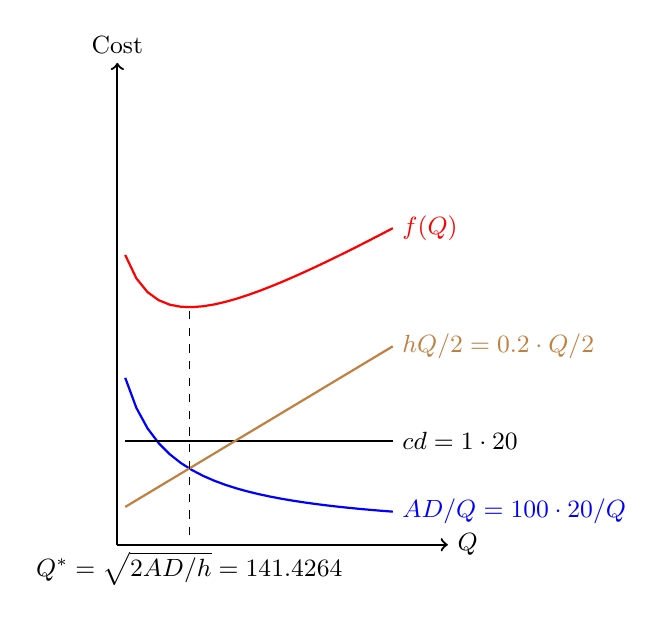
\begin{tikzpicture}[x=0.01cm,y=0.06cm]
\small
\def\c{1} 
\def\K{100} 
\def\h{0.2} 
\def\d{20} 
\pgfmathsetmacro{\Q}{sqrt(2)*sqrt(\K)*sqrt(\d)/sqrt(\h)}
\pgfmathsetmacro{\f}{sqrt(2)*sqrt(\K)*sqrt(\d)*sqrt(\h)+\c*\d}	
\draw[thick,->] (50,-2) -- (470,-2) node[right] {$Q$};
\draw[thick,->] (50,-2) -- (50,100) node[above] {Cost};
\draw[color=blue,thick,domain=60:400] plot (\x,{\d*\K/\x}) node[right] {$AD / Q = \K\cdot\d / Q$};
\draw[color=black,thick,domain=60:400] plot (\x,{\c*\d}) node[right] {$cd = \c\cdot \d$};
\draw[color=brown,thick,domain=60:400] plot (\x,{\h*\x/2}) node[right] {$hQ / 2 = \h\cdot Q / 2$};
\draw[color=red,thick,domain=60:400] plot (\x,{\d*\K/\x+\c*\d+\h*\x/2}) node[right] {$f(Q)$};
\draw (\Q,-1.5) node[below] {$Q^{*} = \sqrt{2AD / h} = \Q$};
\draw[dashed] (\Q,0) -- (\Q,\f);
\end{tikzpicture}
\end{center}

For $A=200$ $c=1$ $h=0.2$ $D=20$:
\begin{center}
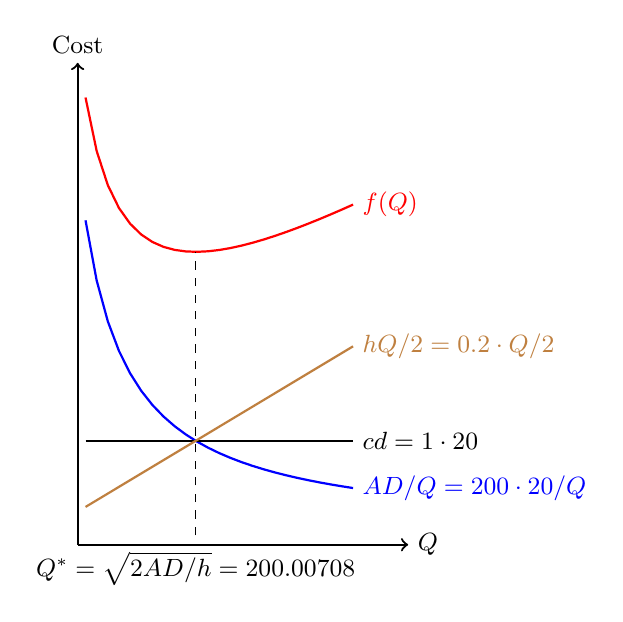
\begin{tikzpicture}[x=0.01cm,y=0.06cm]
\small
\def\c{1} 
\def\K{200} 
\def\h{0.2} 
\def\d{20} 
\pgfmathsetmacro{\Q}{sqrt(2)*sqrt(\K)*sqrt(\d)/sqrt(\h)}
\pgfmathsetmacro{\f}{sqrt(2)*sqrt(\K)*sqrt(\d)*sqrt(\h)+\c*\d}	
\draw[thick,->] (50,-2) -- (470,-2) node[right] {$Q$};
\draw[thick,->] (50,-2) -- (50,100) node[above] {Cost};
\draw[color=blue,thick,domain=60:400] plot (\x,{\d*\K/\x}) node[right] {$AD / Q = \K\cdot\d / Q$};
\draw[color=black,thick,domain=60:400] plot (\x,{\c*\d}) node[right] {$cd = \c\cdot \d$};
\draw[color=brown,thick,domain=60:400] plot (\x,{\h*\x/2}) node[right] {$hQ / 2 = \h\cdot Q / 2$};
\draw[color=red,thick,domain=60:400] plot (\x,{\d*\K/\x+\c*\d+\h*\x/2}) node[right] {$f(Q)$};
\draw (\Q,-1.5) node[below] {$Q^{*} = \sqrt{2AD / h} = \Q$};
\draw[dashed] (\Q,0) -- (\Q,\f);
\end{tikzpicture}
\end{center}

For $A=200$ $c=1$ $h=0.3$ $D=20$:
\begin{center}
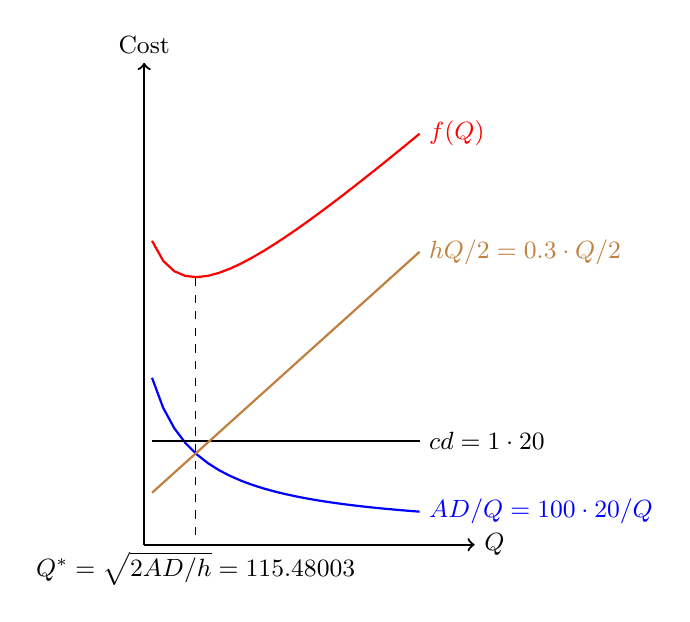
\begin{tikzpicture}[x=0.01cm,y=0.06cm]
\small
\def\c{1} 
\def\K{100} 
\def\h{0.3} 
\def\d{20} 
\pgfmathsetmacro{\Q}{sqrt(2)*sqrt(\K)*sqrt(\d)/sqrt(\h)}
\pgfmathsetmacro{\f}{sqrt(2)*sqrt(\K)*sqrt(\d)*sqrt(\h)+\c*\d}	
\draw[thick,->] (50,-2) -- (470,-2) node[right] {$Q$};
\draw[thick,->] (50,-2) -- (50,100) node[above] {Cost};
\draw[color=blue,thick,domain=60:400] plot (\x,{\d*\K/\x}) node[right] {$AD / Q = \K\cdot\d / Q$};
\draw[color=black,thick,domain=60:400] plot (\x,{\c*\d}) node[right] {$cd = \c\cdot \d$};
\draw[color=brown,thick,domain=60:400] plot (\x,{\h*\x/2}) node[right] {$hQ / 2 = \h\cdot Q / 2$};
\draw[color=red,thick,domain=60:400] plot (\x,{\d*\K/\x+\c*\d+\h*\x/2}) node[right] {$f(Q)$};
\draw (\Q,-1.5) node[below] {$Q^{*} = \sqrt{2AD / h} = \Q$};
\draw[dashed] (\Q,0) -- (\Q,\f);
\end{tikzpicture}
\end{center}

For $A=100$ $c=1$ $h=0.2$ $D=30$:
\begin{center}
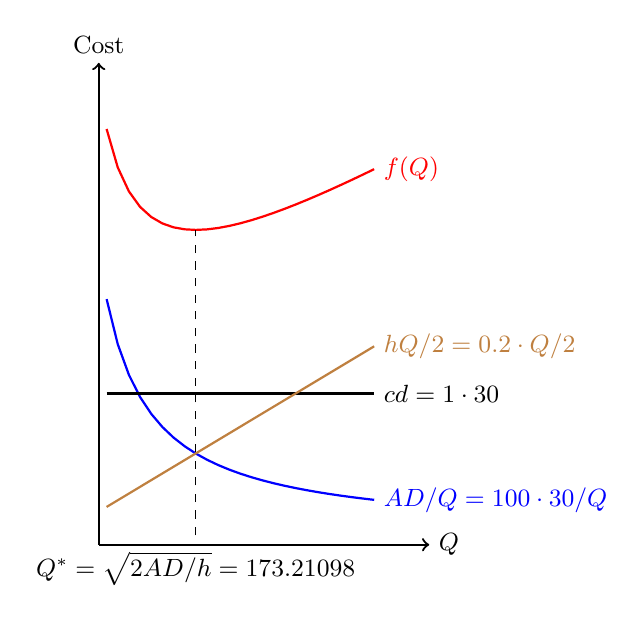
\begin{tikzpicture}[x=0.01cm,y=0.06cm]
\small
\def\c{1} 
\def\K{100} 
\def\h{0.2} 
\def\d{30} 
\pgfmathsetmacro{\Q}{sqrt(2)*sqrt(\K)*sqrt(\d)/sqrt(\h)}
\pgfmathsetmacro{\f}{sqrt(2)*sqrt(\K)*sqrt(\d)*sqrt(\h)+\c*\d}	
\draw[thick,->] (50,-2) -- (470,-2) node[right] {$Q$};
\draw[thick,->] (50,-2) -- (50,100) node[above] {Cost};
\draw[color=blue,thick,domain=60:400] plot (\x,{\d*\K/\x}) node[right] {$AD / Q = \K\cdot\d / Q$};
\draw[color=black,thick,domain=60:400] plot (\x,{\c*\d}) node[right] {$cd = \c\cdot \d$};
\draw[color=brown,thick,domain=60:400] plot (\x,{\h*\x/2}) node[right] {$hQ / 2 = \h\cdot Q / 2$};
\draw[color=red,thick,domain=60:400] plot (\x,{\d*\K/\x+\c*\d+\h*\x/2}) node[right] {$f(Q)$};
\draw (\Q,-1.5) node[below] {$Q^{*} = \sqrt{2AD / h} = \Q$};
\draw[dashed] (\Q,0) -- (\Q,\f);
\end{tikzpicture}
\end{center}
\end{solution}
\end{exercise}


\begin{exercise}
The EOQ formula shows that the optimal order quantity is independent of the unit procurement cost. Why is this is so?  As a consequence, the procurement cost is typically  left out of the analysis.
\begin{solution}
Because we order what we need: Thus, the average cost per unit time is $cD$, i.e., the demand rate $D$ times the cost per unit. Clearly, the procurement cost  cannot have an effect on the optimal order quantity.
\end{solution}
\end{exercise}

\begin{comment}
\begin{exercise} \nvf{This idea is actually wrong. What if inventory is $Q^3$. We have to remove this.}
All the figures suggest that the optimal order quantity is such an order quantity where the ordering and inventory costs per unit time are the same. Is it always the case?


\begin{solution}
Yes. A formal proof can also be provided, but the intuition behind it is more important and it is rather simple. Because average procurement cost per unit time is constant, the cost trade-off lies in ordering and inventory costs per unit time. It is easy to see that the average ordering cost is decreasing in $Q$ and the average holding cost is increasing in $Q$ (see formulas and figures). Therefore, it is always better to choose a $Q$ such that these cost are balanced.
\end{solution}
\end{exercise}
\end{comment}

\begin{exercise}
  It is very important to memorize that the total inventory cost for
  the EOQ model is quite insensitive to the actual order quantity
  $Q$. Show this for the case with $A=100$, $h=0.2$, and $D=20$. What
  happens to the total cost if $Q=60, 80, \ldots 200$?
  \begin{solution}
If we plug in the parameters we obtain from the EOQ formula that $Q^{*} \approx 141.42$ units and $f(Q^{*}) \approx \mathdollar 48.28$. For the other parameters:
\begin{center}
\footnotesize
\begin{tabular}{rrrrr}
\toprule
$Q$     & $AD/Q$  &  $hQ/2$  & $f(Q)$ \\
\midrule
    60    & 33.33 &  6.00  & 59.33 \\
    80    & 25.00 &  8.00  & 53.00 \\
    100   & 20.00 &  10.00 & 50.00 \\
    120   & 16.67 &  12.00 & 48.67 \\
    140   & 14.29 &  14.00 & 48.29 \\
    160   & 12.50 &  16.00 & 48.50 \\
    180   & 11.11 &  18.00 & 49.11 \\
    200   & 10.00 &  20.00 & 50.00 \\
\bottomrule
\end{tabular}
\end{center}
  \end{solution}
\end{exercise}


\begin{exercise}[Implicit Ordering Cost]
For instance,
      suppose we order in quantities of $Q$, e.g., 100 items, what is
      the implied ordering cost?  Well: use the EOQ formula to see
      that this is $A=hQ^2/2D$.  Lets suppose that $h=1$ Euro per year
      per item, and the demand is 100 items per year. Then,
      $A=1(100)^2/(2\cdot 100) = 50$ Euro. Depending on the business
      context this may reasonable, in the order of a delivery cost by
      a truck.
\end{exercise}


In the next set of questions we modify the assumptions of the EOQ model with the aim to investigate how the environment affects the inventory policy.



\subsection{Positive Leadtimes}
\label{sec:variations}

\nvf{introduce inventory position and inventory level}

\begin{exercise}\label{ex:7}
  As a first variation, what would you change/do if the lead time
  is no longer 0, but a positive constant  $L$? Thus, all the other
  assumptions of the EOQ model stay the same, only the lead time
  becomes positive.  In other words, how would you change the EOQ
  policy, and determine when and how to order?

  \begin{solution}
    Since the backlog costs are infinite, backlogging is not
    desirable, hence we order early. The revised ordering policy follows from the graph below.
\begin{center}
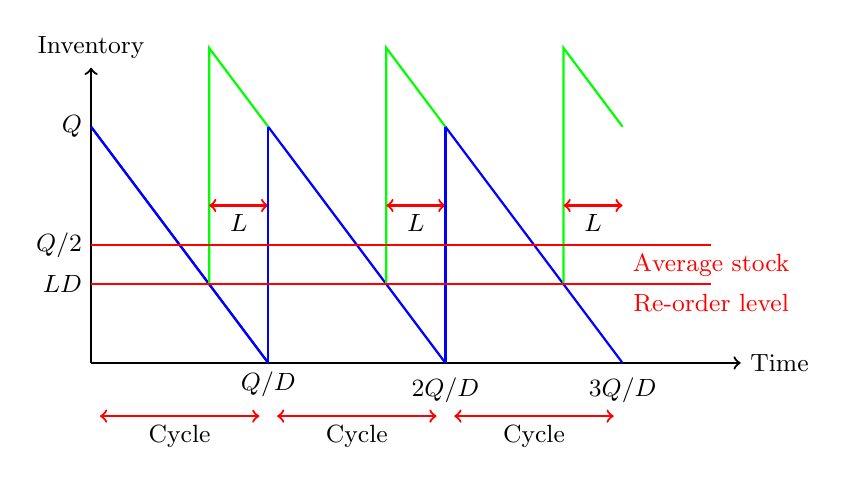
\begin{tikzpicture}[x=0.75cm,y=0.015cm]
\small
\draw[thick,->] (0,0) -- (11,0) node[right] {Time};
\draw[thick,->] (0,0) -- (0,250) node[above] {Inventory};
\draw[] (0,200) -- (0,200) node[left] {$Q$};
\draw[color=blue,thick] (0,200) -- (3,0);
\draw[] (3,0) node[below] {$Q / D$};
\foreach \y in {1,...,3}{
	\draw[color=blue,thick] (3*\y-3,200) -- (3*\y,0);
	\draw[color=green,thick] (3*\y-3+2,200/3) -- (3*\y-3+2,200/3*4) -- (3*\y,200);
	\draw[color=red,thick,<->] (3*\y-3+2,200/3*2) -- (3*\y,200/3*2);
	\draw[] (3*\y-3+2.5,200/3*2) node[below] {$L$};}
\foreach \y in {1,2}{
	\draw[color=blue,thick] (3*\y,0) -- (3*\y,200);}
\foreach \y in {2,3}{
	\draw[] (3*\y,-5) node[below] {\y $Q/D$};}
\draw[] (0,100) node[left] {$Q / 2$};
\draw[color=red,thick] (0,100) -- (10.5,100) node[below] {Average stock};
\draw[] (0,200/3) node[left] {$L D$};
\draw[color=red,thick] (0,200/3) -- (10.5,200/3) node[below] {Re-order level};
\foreach \y in {0,...,2}{
	\draw[color=red,thick,<->] (3*\y+0.15,-45) -- (3*\y+3-0.15,-45);
	\draw[] (3*\y+1.5,-45) -- (3*\y+1.5,-45) node[below] {Cycle};}
\end{tikzpicture}
\end{center}
    
This new policy can be described in a simple way by introducing the
concept of \emph{inventory position}, that is, all stock on-hand plus
the replenishments under way. The green graph above illustrates the
inventory position $\IP$. When $\IP$ hits the lead time demand $L D$,
i.e., the lead time $L$ times the demand $D$, we should order
$Q$. During the lead time $L$ the demand will be met from on-hand
stock. When the replenishment arrives a lead time $L$ later, it
arrives just in time to meet the demand again .

Observe that the cost analysis remains unchanged, as the effect of the lead time is solely on the point in time where a replenishment order is placed, and not on the frequency of orders and/or the actual stock levels. 

  \end{solution}
\end{exercise}

% \begin{exercise}

% How can we decompose leadtime?

% \begin{solution}
% TBD
% \end{solution}
% \end{exercise}

\begin{exercise}
Explain how the inventory policy can be described in presence of a positive lead time. What are its parameters? How does it work?


  \begin{solution}
It is still a very simple policy. It has a single parameter $Q$. It works as follows: place an order of size $Q$ whenever the inventory level hits the level $LD$.
  \end{solution}
\end{exercise}





\subsection{Backlogging}
\label{sec:backlogging}

\begin{exercise}
  What would happen if demand during stock-outs is backordered? 
Sketch the graph of the inventory process if we allow for maximally $B$ units of demand in backlog and we still order some order quantity $Q$. (As we know already know the effect of positive lead times, we take $L=0$ again.)
  \begin{solution}

\begin{center}
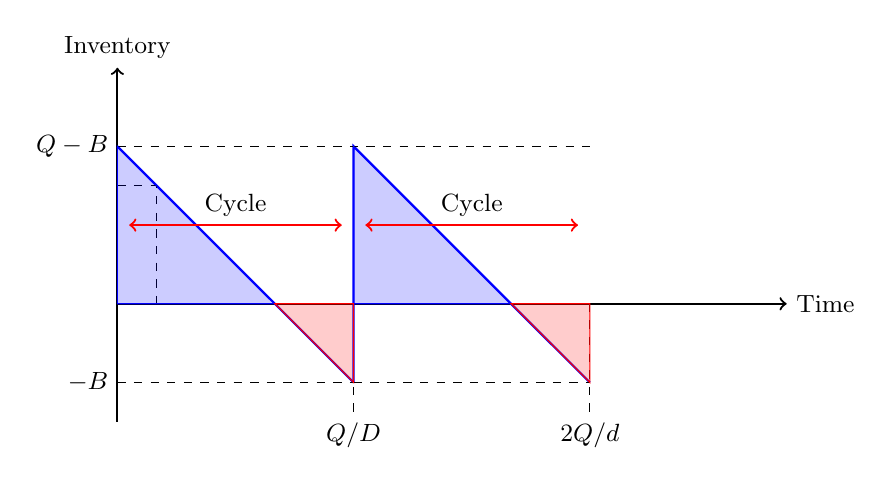
\begin{tikzpicture}[x=1cm,y=0.01cm]
\small

\draw[thick,->] (0,0) -- (8.5,0) node[right] {Time};
\draw[thick,->] (0,-150) -- (0,300) node[above] {Inventory};

\draw[] (0,200) node[left] {$Q - B$};

\draw[color=blue,thick] (0,200) -- (3,-100);

\draw[] (0,-100) node[left] {$-B$};
\draw[dashed] (0,-100) -- (3,-100);

%\draw[] (0,150) node[left] {$Q - B - Dt$};
%\draw[] (0.5,0) node[below] {$t$};
\draw[dashed] (0,150) -- (0.5,150) -- (0.5,0);

%\draw[] (2,0) node[below] {$(Q - B) / d$};

\draw[dashed] (3,0) -- (3,-140) node[below] {$Q / D$};

\draw[color=blue,thick] (3,-100) -- (3,200) -- (6,-100);
%\draw[] (5,0) node[below] {$(2Q - B) / d$};
\draw[dashed] (6,0) -- (6,-140) node[below] {$2Q / d$};
\draw[dashed] (0,200) -- (6,200);
\draw[dashed] (3,-100) -- (6,-100);

\draw [draw=blue,fill=blue,fill opacity=0.2] (0,0) -- (0,200) -- (2,0) -- cycle;
\draw [draw=blue,fill=blue,fill opacity=0.2] (3,0) -- (3,200) -- (5,0) -- cycle;
\draw [draw=red,fill=red,fill opacity=0.2] (2,0) -- (3,-100) -- (3,0) -- cycle;
\draw [draw=red,fill=red,fill opacity=0.2] (5,0) -- (6,-100) -- (6,0) -- cycle;

\foreach \y in {0,1}{
	\draw[color=red,thick,<->] (3*\y+0.15,100) -- (3*\y+3-0.15,100);
	\draw[] (3*\y+1.5,100) node[above] {Cycle};}
\end{tikzpicture}
\end{center}
\end{solution}
\end{exercise}

\begin{exercise}
Let's  assume that the backordering cost is $b>0$ per unit per time, that is, for each customer we pay $b$ per unit time, but $\pi=0$.  If you allow for backorders, will the optimal cost go down or up?  What   will happen to the optimal order quantity $Q$, will it become larger or smaller? 
  \begin{solution}
  Of course we would allow for a bit of backlogging. The
  intuition is this. If we allow for backlogging and order in slightly
  larger quantities, the order cycle becomes longer. Hence, with a bit
  of extra backlogging cost, we can lower the average cost, and make the optimal order quantity a bit larger than for the EOQ model.

As a more theoretical argument,  the cost must become lower: we remove a constraint, where the constraint in the original EOQ is to disallow backorders. 
  \end{solution}
\end{exercise}


\begin{exercise}
  Make a cost model in which we allow for maximally $B$ units of demand in backlog. Show that 
the the average cost is 
\begin{align*}
f(Q,B) 
&= \frac{AD}{Q} + \frac{h(Q-B)^2}{2Q} + \frac{bB^2}{2Q},
\end{align*}
where leave out the procurement cost.
  \begin{solution}

Here, we order $Q$ units every $\frac{Q}{D}$ time units. However, we replenishing inventories when the stock level hits some level $-B$, rather than zero. In each replenishment cycle of length $\frac{Q}{D}$; we spend $\frac{Q-B}{D}$ units of time while having inventories and $\frac{B}{D}$ units of time having stock-outs. 


The total cost for one cycle is the sum of the ordering cost and the inventory (holding and backorder) cost. 

The order cost is $A$ per cycle as we order only once in each cycle. 

The holding cost per cycle is the total area of the blue triangle times $h$, i.e. 
\begin{equation*}
h \frac{\text{height}\cdot\text{base}}{2} = h \frac{(Q-B) \cdot (Q-B)/D}{2} = \frac{h(Q-B)^2}{2D}.
\end{equation*}

The backorder cost per cycle is the total area of the red triangle times $b$, i.e. 
\begin{equation*}
b \frac{\text{height}\cdot\text{base}}{2} = b \frac{B \cdot B/D}{2} = \frac{b B^2}{2D}.
\end{equation*}

The average cost per unit time is this total cost divided by the duration of one cycle $Q/D$. Thus, 
\begin{align*}
f(Q,B) 
&= A \frac{D}{Q} + \frac{h(Q-B)^2}{2D} \frac{D}{Q} + \frac{hB^2}{2D} \frac{D}{Q} \\
&= \frac{AD}{Q} + \frac{h(Q-B)^2}{2Q} + \frac{bB^2}{2Q}.
\end{align*}

\end{solution}
\end{exercise}

\begin{exercise}
What do you get in the result of the previous exercise if you set $B=0$? What value would you choose for $B$ if $b$ is very large? What value for $Q$ would you choose if $h$ is very large? Relate these two cases to an MTO and MTS setting.
  \begin{solution}
For $B=0$  we get the old EOQ result. When $b\gg 0$, we prefer to take $B=0$. When $h\gg0$ then we like to have $Q-B=0$. 

Clearly, we like MTO when $h$ is large, and then $Q=B$, i.e., we produce/order to get rid of the backlog. In the case of MTS, $b$ is typically very large, and then we cover demand from on-hand stock, and $B=0$ preferably.
\end{solution}
\end{exercise}




\begin{exercise}
Explain the inventory policy behind the EOQ model with backlogging. What are its parameters? How does it work?


  \begin{solution}
It is a simple policy. It has two parameters $Q$ and $B$. It works as follows: place an order of size $Q$ whenever the backorder level reaches $B$.
  \end{solution}
\end{exercise}


\begin{exercise}
  Let us consider once again the original EOQ model and imagine a situation where items or ordering
  costs are so high that it is better not to `enter the business' at
  all. Can you find a condition to decide whether to keep inventories
  and satisfy demand or reject all demand and have no inventories?


  \begin{solution}
  
	The EOQ model is based on the assumption that we indeed satisfy the demand in the long term. The reason behind this assumption is our initial idea that it is 'profitable' to stay in the game. We now challenge that initial idea. 
	
	To begin with, we need to introduce an incentive to stay in the game. For instance, a revenue from sales. Let's assume that our selling price for item is $p$. If we satisfy the demand in the long term, we know that our average revenue per unit time would be $pD$. Observe that it works exactly the same way with average procurement cost which was $cD$. The average revenue per unit time is independent of the order quantity. That is, we obtain this revenue regardless of which inventory policy we use. 
	
	Now let's turn back to the question of whether or not to staying in the game. If we stayed in the game and employed the optimal ordering policy; our average revenue would be $pD$ and our average total cost will be $f(Q^*)=\sqrt{2ADh}+cD$. This would lead to a net profit of $(p-c)D-\sqrt{2ADh}$. If this value is positive, or put in other words, if we make profit, then we would stay in the business. 
  \end{solution}
\end{exercise}

\begin{exercise}
Implement $f(Q,B)$ in excel and sketch the cost as a function of $Q$ when $A=100$, $h=0.2$, $D=20$, $b=1$, for the case with $B=0$, $B=10$ and $B=60$.
  Analyze the graphs to see what happens to the  cost and order quantity if you allow for backorders.
  \begin{solution}
\begin{center}
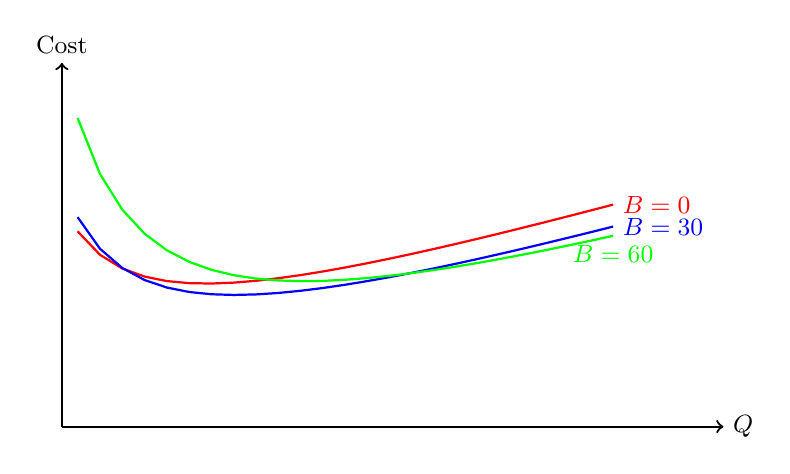
\begin{tikzpicture}[x=0.02cm,y=0.06cm,
declare function = {
f(\Q) = \D*\A/\Q+\h/2*(\Q-\B)/\Q*(\Q-\B)+\b/2*\B/\Q*\B; }
]
\small
\def\A{100} 
\def\h{0.2} 
\def\D{20} 
\def\b{1}
%\def\B{0}
%\pgfmathsetmacro{\f}{sqrt(2)*sqrt(\A)*sqrt(\D)*sqrt(\h)}	
\draw[thick,->] (50,-2) -- (470,-2) node[right] {$Q$};
\draw[thick,->] (50,-2) -- (50,75) node[above] {Cost};
%\draw[color=red,thick,domain=60:400] plot function{\D*\A/x+\h*x/2} node[right] {$B=0$};
%\draw[color=red,thick,domain=60:400] plot (\x,{\D*\A/\x+1*pow(\x,2)}) node[right] {$B=0$};
\def\B{0}
\draw[color=red,thick,domain=60:400] plot (\x,{f(\x)}) node[right] {$B=\B$};
\def\B{30}
\draw[color=blue,thick,domain=60:400] plot (\x,{f(\x)}) node[right] {$B=\B$};
\def\B{60}
\draw[color=green,thick,domain=60:400] plot (\x,{f(\x)}) node[below] {$B=\B$};
% \begin{axis}
% \addplot {f(x)};
% \end{axis}
\end{tikzpicture}
\end{center}


We see that the curve related to $B=30$, i.e., the
blue curve, achieves the lowest point of each of the three graphs.
The minimum of the blue curve is realized a bit to the right of the
minimum of the $B=0$ curve, i.e., the red curve.  Thus, from the
graphs, by setting $B=30$ and $Q$ a bit larger than the optimal value
for the EOQ model, we can lower the cost a bit.
\end{solution}
\end{exercise}

\begin{exercise}
Note that the optimization over $Q$ and $B$ is not as simple as for the EOQ model: we
    now have two `controls' (or degrees of freedom). However, it is still not hard to  show that
 the optimal order quantity,  backorder level and minimal cost take the form
\begin{align*}
Q^* &= \sqrt{\frac{2AD}{h}} \sqrt{\frac{h+b}{b}} \\
B^* &= Q^* \frac{h}{h+b} = , \\
f(Q^*,B^*)  & = \sqrt{2ADh} \sqrt{\frac{b}{h+b}}.
\end{align*}

  \begin{solution}
Use that the average cost function $f(Q,B)$ is differentiable and jointly convex in $Q$ and $B$.
  \end{solution}
\end{exercise}

\begin{exercise}
What happens to the optimal order quantity $Q^*$ in the case $b\gg 1$ or $b \to 0$? How does it compare to the original $Q^*$?

\begin{solution}

 The formula for the optimal order quantity is a slight modification of the formula derived for the no-stock-out case. We simply multiply it with the constant $\sqrt{\frac{h+b}{b}}$. If $b$ is extremely large, then this constant approaches 1 and we have the same optimal order quantity with the no-stock-out case. 

For arbitrary values of $b$ the constant will be larger than 1. Therefore, we can conclude that the optimal order quantity will be higher as compared to the no-stock-out case and the difference will be larger for smaller values of $b$. 
\end{solution}
\end{exercise}


\begin{exercise}
What happens to the optimal backlog quantity $B^*$ in the case $b\gg 1$ or $b \to 0$? 
\begin{solution}
 The optimal backorder level is a constant fraction of the order quantity. This fraction $\frac{h}{h+b}$ in fact reflects on the trade-off between the holding and backorder costs. For instance, if $b=9h$, then the backorder level should be 10\% of the order quantity. Furthermore, this immediately means that you should spend 10\% of the time with stock-outs and the remaining 90\% with inventories. 

If we put together this with our previous observation; we can conclude that a small backorder cost leads to (1) large order quantities, and (2) backorder levels being even larger fractions of the order quantities. 
\end{solution}
\end{exercise}


\begin{exercise}
What happens to the optimal average cost in the case $b\gg 1$ or $b \to 0$? 
\begin{solution}
The optimal average cost can also be obtained with a slight modification of the original one. The procurement costs remain the same but we simply multiply the inventory costs with the constant $\sqrt{\frac{b}{h+b}}$. If $b$ is extremely large, then this constant approaches 1 and we have the same optimal cost with the no-stock-out case. 

For arbitrary values of $b$ the constant will be smaller than 1. Therefore, we can conclude that the optimal average cost will be lower as compared to the no-stock-out case and the difference will be larger for smaller values of $b$. 
\end{solution}
\end{exercise}


\begin{exercise}
Let's numerically analyze these effects. Implement the formulas in excel and analyze numericall the case with $A=100$, $h=0.2$, $c=1$,  $D=20$ and  $b=0.5,1.0,\ldots 10.0$.

\begin{solution}
We know for the no-stockout case that if we plug in the parameters we obtain from the EOQ formula that $Q^{*} \approx 141.42$ units and $f(Q^{*}) \approx \mathdollar 48.28$. For different values of $b$ we obtain the results in the table below. 

\begin{center}
    \begin{tabular}{rrrr}
    \toprule
    $b$ & $Q^*$ & $B^*$ & $f(Q^*,B^*)$ \\
    \midrule
    0.5   & 167.33 & 47.81 & 43.90 \\
    1.0   & 154.92 & 25.82 & 45.82 \\
    1.5   & 150.55 & 17.71 & 46.57 \\
    2.0   & 148.32 & 13.48 & 46.97 \\
    2.5   & 146.97 & 10.89 & 47.22 \\
    3.0   & 146.06 & 9.13  & 47.39 \\
    3.5   & 145.41 & 7.86  & 47.51 \\
    4.0   & 144.91 & 6.90  & 47.60 \\
    4.5   & 144.53 & 6.15  & 47.68 \\
    5.0   & 144.22 & 5.55  & 47.74 \\
    5.5   & 143.97 & 5.05  & 47.78 \\
    6.0   & 143.76 & 4.64  & 47.82 \\
    6.5   & 143.58 & 4.29  & 47.86 \\
    7.0   & 143.43 & 3.98  & 47.89 \\
    7.5   & 143.29 & 3.72  & 47.91 \\
    8.0   & 143.18 & 3.49  & 47.94 \\
    8.5   & 143.08 & 3.29  & 47.96 \\
    9.0   & 142.98 & 3.11  & 47.98 \\
    9.5   & 142.90 & 2.95  & 47.99 \\
    10.0  & 142.83 & 2.80  & 48.01 \\
	1000.0	& 141.44 & 0.03	& 48.28 \\
    \bottomrule
    \end{tabular}%
\end{center}

Note that all numbers are in line with our expectations. For instance, for increasing values of backorder cost, $Q^*$ and $B^*$ both decrease and the optimal average cost increases. Notice that the last row stands for a 'very large' backorder cost. Here, we see that the optimal backorder level is almost zero, and the optimal order quantity and the optimal average cost are almost the same with no-stock-out case. 
\end{solution}
\end{exercise}

\subsection{Lost Sales}
\label{sec:lost-sales}

\begin{exercise}We can also decide to reject demand rather than
  backlog it. Can you sketch the consequences on the behavior of the
  inventory level, assuming that the cycle length is $T$. (Since we do not order when the inventory hits zero, as in the EOQ case, or when the backlog level becomes $B$, as in the case with backlogging, we need to consider another rule to trigger a replenishment order. Hence, we assume that we order after every $T$ time periods.)

  \begin{solution}
    The influence on the cost is qualitatively easy. Once again we
    relax a constraint, hence it must be possible to reduce the
    average cost. 

If we order every $T$ times, than we get the following graph. Note, after time $Q/D$ the inventory is empty. The demand arriving during the interval $[Q/D, T]$ is lost. 
\begin{center}
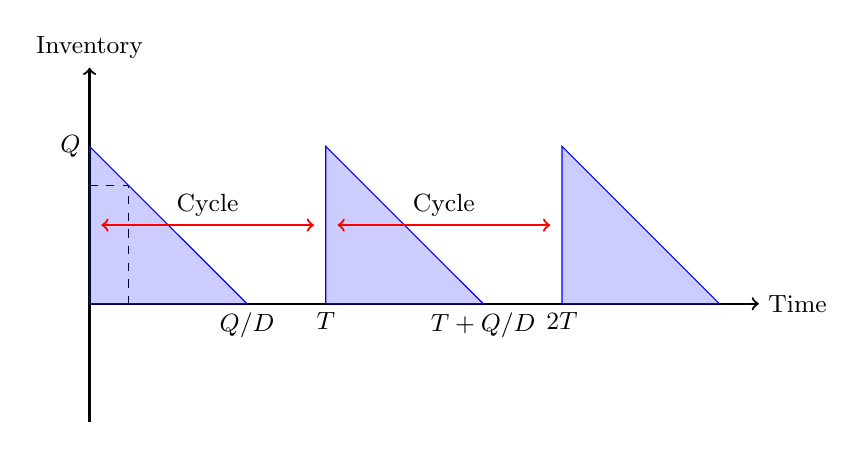
\begin{tikzpicture}[x=1cm,y=0.01cm]
\small

\draw[thick,->] (0,0) -- (8.5,0) node[right] {Time};
\draw[thick,->] (0,-150) -- (0,300) node[above] {Inventory};

\draw[] (0,200) node[left] {$Q$};

%\draw[color=blue,thick] (0,200) -- (3,-100);


%\draw[] (0,150) node[left] {$Q - B - Dt$};
%\draw[] (0.5,0) node[below] {$t$};
\draw[dashed] (0,150) -- (0.5,150) -- (0.5,0);

%\draw[] (2,0) node[below] {$(Q - B) / d$};

\draw[] (2,0) node[below] {$Q/D$};
\draw[] (3,0) node[below] {$T$};

%\draw[color=blue,thick] (3,-100) -- (3,200) -- (6,-100);
%\draw[] (5,0) node[below] {$(2Q - B) / d$};
\draw[] (5,0) node[below] {$T+Q/D$};
\draw[] (6,0) node[below] {$2T$};
%\draw[dashed] (0,200) -- (6,200);
%\draw[dashed] (3,-100) -- (6,-100);

\draw [draw=blue,fill=blue,fill opacity=0.2] (0,0) -- (0,200) -- (2,0) -- cycle;
\draw [draw=blue,fill=blue,fill opacity=0.2] (3,0) -- (3,200) -- (5,0) -- cycle;
\draw [draw=blue,fill=blue,fill opacity=0.2] (6,0) -- (6,200) -- (8,0) -- cycle;

\foreach \y in {0,1}{
	\draw[color=red,thick,<->] (3*\y+0.15,100) -- (3*\y+3-0.15,100);
	\draw[] (3*\y+1.5,100) node[above] {Cycle};}
\end{tikzpicture}
\end{center}
\end{solution}
\end{exercise}

\begin{exercise} Find a formula for the average cost when the cycle duration is $T$.
  \begin{solution}
The average cost is the ordering cost plus the inventory cost plus the
cost of lost demand. We already analyzed the cost of the first two
terms. The loss cost is related to all demand lost between the time
$Q/D$ (i.e., the timer it takes the demand to consume $Q$) and the
next order moment $T$. The lost demand is
$DT-Q$. Thus, the average cost becomes
\begin{align*}
  f(Q) 
&= \frac A T + \frac h2 \frac{Q\cdot Q/D}{T}+k \frac{DT-Q}T \\
&= \frac A T + \frac{hQ^2}{2DT}+k \left(D-\frac Q T\right). 
\end{align*}
\end{solution}
\end{exercise}

\begin{uncomment}
  
\begin{exercise}[\faRocket] For what $T$ is the  average cost for a model with loss lower than the EOQ cost (without loss or backlogging).
  \begin{solution}
Lets subtract the average cost from EOQ model from the average cost of loss model. Then we get
  \begin{align*}
&\text{cost loss model } - \text{cost EOQ} \\
&=\frac A T + \frac{hQ^2}{2DT}+k\left(D-\frac Q T\right)  - \frac{A D}{Q} - \frac{h Q}{2}.
  \end{align*}
We can simplify this as follows: 
\begin{align*}
&\frac A T + \frac{hQ^2}{2DT}+k\left(D-\frac Q T\right)  - \frac{A D}{Q} - \frac{h Q}{2} \\
&= A \left(\frac 1 T - \frac D Q\right) + \frac{h Q} 2 \left(\frac{Q}{DT}-1\right)+k\left(D-\frac Q   T\right) \\
&= \frac A Q \left(\frac Q T - D \right) + \frac{h Q} {2D} \left(\frac{Q}{T}- D \right)+k\left(D-\frac Q  T\right)  \\
&= \left(\frac A Q + \frac{h Q} {2D} -k \right) \left(\frac{Q}{T}- D \right) \\
&= \left(\frac A Q + \frac{h Q} {2D} -k \right) \left(Q- T D \right)\frac 1 T. \\
%&= \left(\frac{AD} Q + \frac{h Q} {2} -k D \right) \left(\frac{Q}{T D}- 1 \right).
\end{align*}
This was quite a bit of work, but the result is very interesting. 

First consider the term $Q-T D$. If $Q > T D$, we order more than we consume during a cycle, and the inventory would become even larger. Hence, necessarily $Q\leq T D$, which implies that $Q-T D\leq 0$. 

From the above we can then conclude that the cost of system with loss is higher than the system with inventory and operating under the EOQ policy with order quantity $Q$  when
\begin{equation*}
  \frac{AD} Q + \frac{h Q} {2} < k D.
\end{equation*}
However, this condition comes down to requiring that dropping all demand at a cost $kD$ must be less than holding inventory. In other words, if it is interesting to lose part of the demand, it is in fact best to reject all demand altogether. Otherwise, it is best to prevent loss. 

So, why is that? From the above there seem to be two alternatives,
either order the EOQ and don't reject any demand, or order nothing and
reject all demand.  So, let's trace back the entire analysis.  Indeed,
if we decide to order items and keep them in inventory to satify
demand, then the cost of this must be smaller than the cost of losing
demand. For otherwise, we would simply not be in this business
anyway. So, all in all, this is entirely logical (in hindsight): If
orders are so profitable that you are prepared to keep inventories, it
simply can't be optimal to lose demand. If, however, keeping
inventories is too expensive, it must be optimal not to participate at
all.

Note that this argument is only valid for the case in which everything
is deterministic. In case of stochastic demand, we'll see that
the conclusion changes.
  \end{solution}
\end{exercise}
\end{uncomment}

\begin{comment}
  We need to replace $D$ by $d$, as we consider deterministic demand here.
\end{comment}

% \begin{exercise}We can also decide to reject demand rather than
%   backlog it. Can you sketch the consequences on the behavior of the
%   inventory level?  What happens to the order quantity $Q$?  What are
%   the consequences in terms of cost, does it become lower or higher?
%   \begin{solution}
%     The influence on the cost is qualitatively easy. Once again we
%     relax a constraint, hence it must be possible to reduce the
%     average cost. Again, we are trying to find out by how much. 

%     Let's assume we order every $T$ periods.

% \begin{center}
% \begin{tikzpicture}[x=1cm,y=0.01cm]
% \small

% \draw[thick,->] (0,0) -- (8.5,0) node[right] {Time};
% \draw[thick,->] (0,-150) -- (0,300) node[above] {Inventory};

% \draw[] (0,200) node[left] {$Q$};

% %\draw[color=blue,thick] (0,200) -- (3,-100);


% %\draw[] (0,150) node[left] {$Q - B - Dt$};
% %\draw[] (0.5,0) node[below] {$t$};
% \draw[dashed] (0,150) -- (0.5,150) -- (0.5,0);

% %\draw[] (2,0) node[below] {$(Q - B) / d$};

% \draw[] (2,0) node[below] {$Q/D$};
% \draw[] (3,0) node[below] {$T$};

% %\draw[color=blue,thick] (3,-100) -- (3,200) -- (6,-100);
% %\draw[] (5,0) node[below] {$(2Q - B) / d$};
% \draw[] (5,0) node[below] {$T+Q/D$};
% \draw[] (6,0) node[below] {$2T$};
% %\draw[dashed] (0,200) -- (6,200);
% %\draw[dashed] (3,-100) -- (6,-100);

% \draw [draw=blue,fill=blue,fill opacity=0.2] (0,0) -- (0,200) -- (2,0) -- cycle;
% \draw [draw=blue,fill=blue,fill opacity=0.2] (3,0) -- (3,200) -- (5,0) -- cycle;
% \draw [draw=blue,fill=blue,fill opacity=0.2] (6,0) -- (6,200) -- (8,0) -- cycle;

% \foreach \y in {0,1}{
% 	\draw[color=red,thick,<->] (3*\y+0.15,100) -- (3*\y+3-0.15,100);
% 	\draw[] (3*\y+1.5,100) node[above] {Cycle};}
% \end{tikzpicture}
% \end{center}

% The average cost is the ordering cost plus the inventory cost plus the
% cost of lost demand. We already analyzed the cost of the first two
% terms. The loss cost is related to all demand lost between the time
% $Q/D$ (i.e., the timer it takes the demand to consume $Q$) and the
% next order moment $T$. The lost demand is
% $DT-Q$. Thus, the average cost becomes
% \begin{equation*}
%   \begin{split}
%   f(Q) 
% &= \frac A T + \frac h2 \frac{Q\cdot Q/D}{T}+k \frac{DT-Q}T \\
% &= \frac A T + \frac{hQ^2}{2DT}+k (D-\frac QT). 
%   \end{split}
% \end{equation*}

% Take $A=100$, $h=0.2$, $D=20$, $k=1$. As a first attempt, take $T=D/Q^*$ (for the EOQ quantity $Q^*$.) Since $Q^* \approx 141$ and $D=200$, we take $T=200/141\approx 1.4$. 
% (This is were I made my first mistake, I copied the wrong numbers.)

% \begin{center}
% \begin{tikzpicture}[x=0.02cm,y=0.06cm,
% declare function = {
% f(\Q) = \A/\T+\h/2*\Q/\D*\Q/\T+\k*(\D*\T-\Q); }
% ]
% \small
% \def\A{100} 
% \def\h{0.2} 
% \def\D{20} 
% \def\k{1}
% %\pgfmathsetmacro{\f}{sqrt(2)*sqrt(\A)*sqrt(\D)*sqrt(\h)}	
% \draw[thick,->] (50,-2) -- (470,-2) node[right] {$Q$};
% \draw[thick,->] (50,-2) -- (50,75) node[above] {Cost};
% \def\T{1.2}
% \draw[color=blue,thick,domain=60:400] plot (\x,{f(\x)}) node[right] {$T=\T$};
% \def\T{1.5}
% \draw[color=red,thick,domain=60:400] plot (\x,{f(\x)}) node[right] {$T=\T$};
% \def\T{2.0}
% \draw[color=red,thick,domain=60:400] plot (\x,{f(\x)}) node[right] {$T=\T$};
% \end{tikzpicture}
% \end{center}

% Now I wonder why the graph for $T=2$ becomes negative. I guess I did
% something wrong, but what?  First I'm checked the cost function. The
% only component that can give negative values is
% $k(DT-Q)$. (As it turned out, I also copied the formula
%   incorrectly.) So, when the cost is negative,
% I must be considering a combination of $Q$, $D$ and $T$ such that this
% term is negative. This only happens when $Q>DT$. But this is strange,
% because when $Q>DT$, I am ordering more than the demand that occurs
% between two ordering moments, i.e., during the time interval of length
% $T$. Clearly then, we must require that $T>Q/D$, which makes
% sense. Rechecking also my above estimate for $T$, I notice that I made
% stupid algebraic error. It should have been $T=Q^*/D$. For some reason
% I also used $D=200$ while it should have been $D=20$. So, let's make a
% next attempt with $T=140/20=7$,  use that $Q<DT$, and repair the implementation of the cost function it self (You can't see this in this document, but it is in the source.)

% \begin{center}
% \begin{tikzpicture}[x=0.02cm,y=0.06cm,
% declare function = {
% f(\Q) = \A/\T+\h/2*\Q/\D*\Q/\T+\k*(\D-\Q/\T); }
% ]
% \small
% \def\A{100} 
% \def\h{0.2} 
% \def\D{20} 
% \def\k{1}
% %\pgfmathsetmacro{\f}{sqrt(2)*sqrt(\A)*sqrt(\D)*sqrt(\h)}	
% \draw[thick,->] (50,-2) -- (470,-2) node[right] {$Q$};
% \draw[thick,->] (50,-2) -- (50,75) node[above] {Cost};
% \def\T{7}
% \draw[color=blue,thick,domain=60:\D*\T] plot (\x,{f(\x)}) node[right] {$T=\T$};
% \def\T{8}
% \draw[color=red,thick,domain=60:\D*\T] plot (\x,{f(\x)}) node[right] {$T=\T$};
% \def\T{6}
% \draw[color=red,thick,domain=60:\D*\T] plot (\x,{f(\x)}) node[right] {$T=\T$};
% \end{tikzpicture}
% \end{center}

% This is too bad: my plotting tool (TikZ) is failing on me, the scales
% of the axes are not ok, and I can't read what function belongs to what
% graph. In fact, I am now entirely fed up with TikZ, and move to
% gnuplot (the tried and tested powertool when it comes to making
% plots. With gnuplot I managed to solve the problems in ten minutes. )

% \begin{center}
%   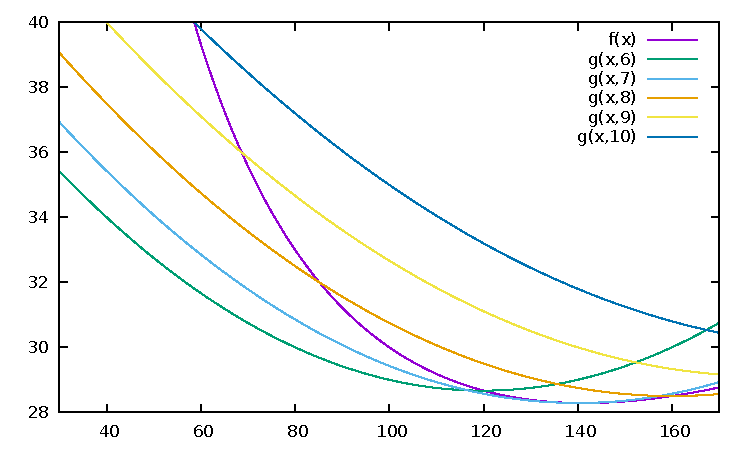
\includegraphics{figures/eoq_loss_0_2}
% \end{center}

% The situation with $k=0.2$. The $f$ is the graph of the EOQ model, the
% $g(x,6)$ is the graph of the cost of the model with loss and with
% $T=6$, the $x$ corresponds to the order size $Q$; likewise $g(x,7)$ is
% the cost for $T=7$ and so on. We now clearly see that none of the
% models with loss achieves a lower cost than the EOQ model with optimal order quantity. 

% \begin{center}
%   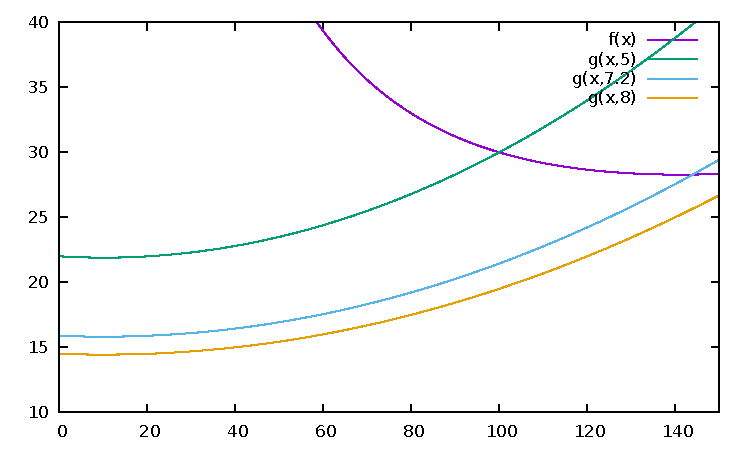
\includegraphics{figures/eoq_loss_0_1}
% \end{center}

% The situation with $k=0.1$. We now see that when rejecting demand is
% pretty cheap, it is best not to order anything: when $Q=0$ the cost is
% minimal, hence rejecting all demand seems to be optimal. This is
% definitely unexpected!

% So, why is that? From the above there seem to be two alternatives,
% either order the EOQ and don't reject any demand, or order nothing and
% reject all demand.  So, let's trace back the entire analysis.  Indeed,
% if we decide to order items and keep them in inventory to satify
% demand, then the cost of this must be smaller than the cost of losing
% demand. For otherwise, we would simply not be in this business
% anyway. So, all in all, this is entirely logical (in hindsight): If
% orders are so profitable that you are prepared to keep inventories, it
% simply can't be optimal to lose demand. If, however, keeping
% inventories is too expensive, it must be optimal not to participate at
% all.

% Note that this argument is only valid for the case in which everything
% is deterministic. In case of stochastic demand, we'll see that
% everything changes.

% % If we
% % reject all demand, then the average cost rate must be $k D$. If, on
% % the other hand, we don't want to reject all demand, we order an amount
% % $Q$. The cost of ordering is:
% % \begin{equation*}
% %   \frac A T + \frac{hQ^2}{2DT} - \frac{k Q}{T}.
% % \end{equation*}
% % Therefore, when this is negative, the overall cost must
% % decrease. Thus, if
% % \begin{equation*}
% %   \frac A T + \frac{hQ^2}{2DT}  < \frac{k Q}{T},
% % \end{equation*}
% % we must be better off by ordering some amount $Q$. Now it appears that
% % all components in this equation are divided by $T$. Removing this
% % leads to
% % \begin{equation*}
% %   A + \frac{hQ^2}{2D}  < k Q.
% % \end{equation*}
% % But now we see that the cost benefit of ordering $Q$ is independent of
% % $T$!
%   \end{solution}
% \end{exercise}




\begin{exercise}[\faRocket]
  Continuing on the above question, it might be that items or ordering
  costs are so high that it is better not to `enter the business' at
  all. Can you find a condition to decide whether to keep inventories
  and satisfy demand or reject all demand and have no inventories?
  \begin{solution}
    The cost rate of dropping all demand is $kD$. The cost rate of keeping inventories is, under the EOQ model,  and using that the optimal order quantity $Q^* = \sqrt{2AD/h}$, 
    \begin{align*}
      f(Q^*)
 &= A \frac{D}{Q^*} + \frac h 2 Q \\
 &= A \frac{D}{\sqrt{2AD/h}} + \frac h 2 \sqrt{\frac{2AD}h} \\
 &= A D \sqrt{\frac{h} {2AD}} + \frac h 2 \sqrt{\frac{2AD}h} \\
 &=  \sqrt{\frac {AhD}{2}} + \sqrt\frac{ADh}2 \\
 &=  2\sqrt{\frac {AhD}{2}} \\
 &=  \sqrt{2AhD}.
    \end{align*}
When the cost rate of rejecting demand is lower than the cost rate of keeping inventories, we reject the demand, that is, when
\begin{equation*}
kD < \sqrt{2AhD}.
\end{equation*}
We can simplity this a bit to $k^2D^2 < 2AhD$, from which we get
\begin{equation*}
  k^2 D < 2 A h.
\end{equation*}
Thus, when the demand is really small, or the reject cost $k$ is
small, we reject demand. 
  \end{solution}
\end{exercise}

\subsection{Discounting}
\label{sec:discounting}



\begin{exercise}
In many practical environments, there is economies of scale in ordering due to quantity discounts. How would this affect the EOQ model?


\begin{solution}
In presence of quantity discounts, we have an incentive to order more since the unit procurement cost decreases with the order size. This can be conceptualized by re-writing procurement cost as a function of the order quantity. There is also an interesting point that relates to the holding costs. It is often assumed that the unit holding cost is a fraction of the unit procurement cost. For instance, the holding cost per year is 30\% of the procurement cost. In case of quantity discounts, this implies that the holding cost is also a function of the order quantity. 
\end{solution}
\end{exercise}

\begin{exercise}
What are the most common discounting schemes? How do they work?


\begin{solution}
There are two common discounting schemes: all-unit discounts and incremental discounts. We discuss them below by means of examples. 

To emphasize the differences between these schemes, we make use a total procurement cost function $c(Q)$, i.e. we pay $c(Q)$ in total if we buy $Q$ units. The shape of $c(Q)$ obviously depends on the discounting scheme.

\paragraph{All-unit discounts} In this example, we have all-unit discounting with three discount intervals; $[0,100)$ interval with price \$1, $[100,200)$ interval with price \$0.8, and $[200,\infty)$ interval with price \$0.6. The discount is applied to all units. For instance, if we buy 120 items, then we pay in total $120\cdot 0.8=\$96$. The total procurement cost function $c(Q)$ of this discounting scheme is illustrated in Figure~\ref{fig:allunit}.

\begin{figure}[htbp]
\centering
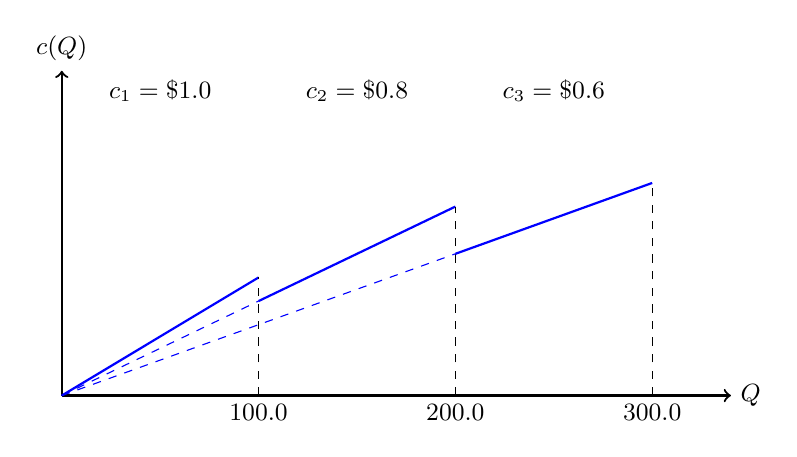
\begin{tikzpicture}[x=0.025cm,y=0.015cm]
\small
\draw[thick,->] (0,0) -- (340,0) node[right] {$Q$};
\draw[thick,->] (0,0) -- (0,275) node[above] {$c(Q)$};
\def\w{100}
\foreach \n/\a in {1/1.0,2/0.8,3/0.6}{
	\pgfmathsetmacro{\s}{(\n-1)*\w}	
	\pgfmathsetmacro{\e}{\n*\w}
	\draw[thick,color=blue,domain=\s:\e] plot (\x,{\a*\x});
	\draw[dashed,color=blue,domain=0:{\s+0.01}] plot (\x,{\a*\x});
	\draw[] (\e,0) -- (\e,0) node[below] {$\e$};
	\draw[dashed] (\e,0) -- (\e,\e*\a);
	\draw[] ({(\s+\e)/2},275) -- ({(\s+\e)/2},275) node[below] {$c_{\n} = \mathdollar\a$};}
\end{tikzpicture}
\caption{All-unit discounts}
\label{fig:allunit}
\end{figure}


\paragraph{Incremental discounts} In this example, we have incremental discounting with exactly the same discount intervals from the previous example. The difference here is that the discount is applied by parts. That is, we pay \$1 per unit for the part of the order that is below 100, we pay \$0.8 for the part of the order that is between 100 and 200, and we pay \$0.6 for the part of the order that is above 200. For instance, if we buy 120 items, then we pay in total $100\cdot 1 + 20 \cdot 0.8=116$. The total procurement cost function $c(Q)$ of this discounting scheme is illustrated in Figure~\ref{fig:incremental}.

\begin{figure}[htbp]
\centering
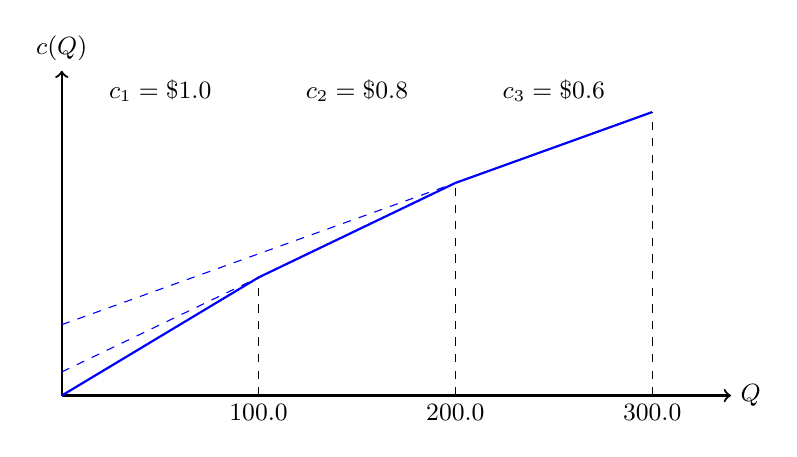
\begin{tikzpicture}[x=0.025cm,y=0.015cm]
\small
\draw[thick,->] (0,0) -- (340,0) node[right] {$Q$};
\draw[thick,->] (0,0) -- (0,275) node[above] {$c(Q)$};
\def\w{100}
\pgfmathsetmacro{\b}{0}
\foreach \n/\a/\b in {1/1.0/0,2/0.8/20,3/0.6/60}{
	\pgfmathsetmacro{\s}{(\n-1)*\w}	
	\pgfmathsetmacro{\e}{\n*\w}
	\draw[thick,color=blue,domain=\s:\e] plot (\x,{\a*\x+\b});
	\draw[dashed,color=blue,domain=0:{\s+0.01}] plot (\x,{\a*\x+\b});
	\draw[] (\e,0) -- (\e,0) node[below] {$\e$};
	\draw[dashed] (\e,0) -- (\e,\e*\a+\b);
	\draw[] ({(\s+\e)/2},275) -- ({(\s+\e)/2},275) node[below] {$c_{\n} = \mathdollar\a$};}
\end{tikzpicture}
\caption{Incremental discounts}
\label{fig:incremental}
\end{figure}
\end{solution}
\end{exercise}

\begin{exercise}
How can we integrate different discounting schemes into the EOQ model? How would they change the resulting policy?


\begin{solution}
Let us first re-write the EOQ cost function (keeping in mind that the holding cost is a fraction of the procurement cost). 
\begin{align*}
f(Q) 
& = \frac{AD}{Q} + cD + \frac{hQ}{2} \\
& = \frac{AD}{Q} + cD + \frac{\alpha cQ}{2} \quad (h = \alpha c) 
\end{align*}

In the following, we discuss the implications of all-unit discounts and incremental discounts on the cost function above. For convenience, we will assume that there are $m$ intervals; 1st interval $[0,Q_1)$, 2nd interval $[Q_1,Q_2)$, and finally $m$th interval $[Q_{m-1},\infty)$. Also, we will let $c_n$ be the price associated with the $n$th interval. 

\paragraph{All-unit discounts}

In case of all-unit discounts, we can write the cost function by conditioning on the order quantity intervals as follows:
\begin{equation*}
f(Q) = 
\begin{cases}
f_1(Q) = \frac{AD}{Q} + c_1D + \frac{\alpha c_1 Q}{2} & \text{if } 0 \leq Q < Q_1 \\
f_2(Q) = \frac{AD}{Q} + c_2D + \frac{\alpha c_2 Q}{2} & \text{if } Q_1 \leq Q < Q_2 \\
\ldots \\
f_m(Q) = \frac{AD}{Q} + c_mD + \frac{\alpha c_m Q}{2} & \text{if } Q_{m-1} \leq Q 
\end{cases}
\end{equation*}

Here, we have a cost function $f_n(Q) = \frac{AD}{Q} + c_nD + \frac{\alpha c_n Q}{2}$ for each interval $n$ which only applies if the order quantity $Q$ is in $[Q_{n-1},Q_n)$. This function has the same mathematical properties with the original EOQ formula. Therefore, we know that $f_n(Q)$ is minimized at $Q^*_n=\sqrt{\frac{2AD}{\alpha c_n}}$ and its minimum value is $f_n(Q^*_n)=\sqrt{2AD\alpha c_n}+c_n D$.

Let us illustrate this by once again considering the example from the previous exercise where $c_1=1.0$, $c_2=0.8$, $c_3=0.6$, $Q_1=100$, and $Q_2=200$. We further let $A=100$, $D=20$, and $\alpha=0.2$. Then we have 
\begin{equation*}
f(Q) = 
\begin{cases}
f_1(Q) = \frac{2000}{Q} + 20 + 0.10 Q & \text{if } 0 \leq Q < 100 \\
f_2(Q) = \frac{2000}{Q} + 16 + 0.08 Q & \text{if } 100 \leq Q < 200 \\
f_3(Q) = \frac{2000}{Q} + 12 + 0.06 Q & \text{if } 200 \leq Q 
\end{cases}
\end{equation*}
and we also know $Q^*_1\approx 141.42$, $Q^*_2\approx 158.11$, and $Q^*_3\approx 182.57$. 

In the Figure~\ref{fig:avgcost_allunit} we draw all these functions.

\begin{figure}[htbp]
\centering
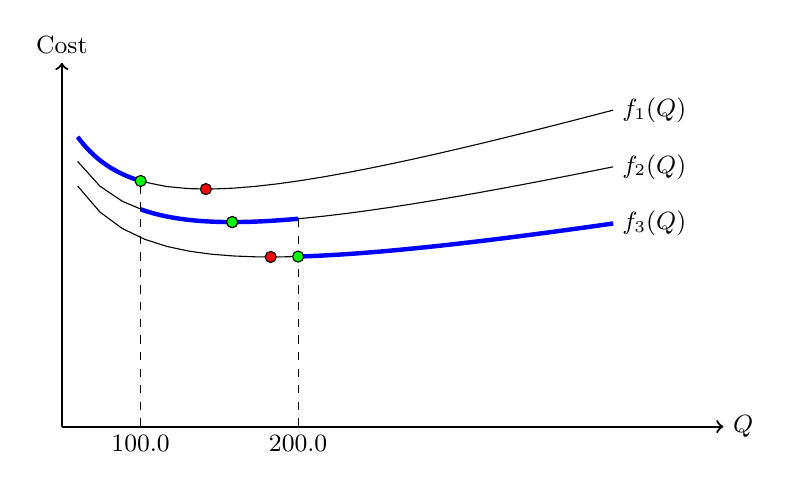
\begin{tikzpicture}[x=0.02cm,y=0.06cm]
\small
\def\c{1} 
\def\K{100} 
\def\h{0.2} 
\def\d{20} 
\def\alpha{0.2}
\def\w{100}
\draw[thick,->] (50,-2) -- (470,-2) node[right] {$Q$};
\draw[thick,->] (50,-2) -- (50,75) node[above] {Cost};
\foreach \n/\c in {1/1.0,2/0.8,3/0.6} {
	\pgfmathsetmacro{\h}{\alpha*\c}	
	\pgfmathsetmacro{\Q}{sqrt(2)*sqrt(\K)*sqrt(\d)/sqrt(\h)}
	\pgfmathsetmacro{\f}{sqrt(2)*sqrt(\K)*sqrt(\d)*sqrt(\h)+\c*\d}	
	\pgfmathsetmacro{\s}{(\n-1)*\w}	
	\pgfmathsetmacro{\e}{\n*\w}

	\draw[domain=60:400] plot (\x,{\d*\K/\x+\c*\d+\h*\x/2}) node[right] {$f_{\n}(Q)$};

	\ifnum\n<3
		\draw[color=blue,ultra thick,domain={max(60,\s}:\e] plot (\x,{\d*\K/\x+\c*\d+\h*\x/2});
		\draw[dashed] (\e,-2) -- (\e,{\d*\K/\e+\c*\d+\h*\e/2});
		\draw (\e,-2) node[below] {$\e$};
	\else
		\draw[color=blue,ultra thick,domain={max(60,\s}:400] plot (\x,{\d*\K/\x+\c*\d+\h*\x/2});
	\fi

	\draw [fill=red] (\Q,\f) circle (2pt);

	\pgfmathparse{int(\Q-\s)}
	\ifnum \pgfmathresult < 0
		\draw [fill=green] (\s,{\d*\K/\s+\c*\d+\h*\s/2}) circle (2pt);
	\fi
	\pgfmathparse{int(\Q-\e)}
	\ifnum \pgfmathresult > 0
		\draw [fill=green] (\e,{\d*\K/\e+\c*\d+\h*\e/2}) circle (2pt);
	\fi
	\pgfmathparse{int((\Q-\e)*(\Q-\s))}
	\ifnum \pgfmathresult < 0
		\draw [fill=green] (\Q,\f) circle (2pt);
	\fi
}
\end{tikzpicture}
\caption{All-unit discounts -- average costs}
\label{fig:avgcost_allunit}
\end{figure}


What we observe here is the following.
\begin{itemize}
\item $f_1(Q)$: This function applies in the $[0,100)$ interval (blue area). It's optimal point is at $141.42$. This point does not fall into function's interval (that's why it is a red dot). Because the function is convex and it's optimal point is to the right of the interval, the minimum point that falls into function's interval is 100 (green dot) which gives a cost of \$50. 
\item $f_2(Q)$: This function applies in the $[100,200)$ interval (blue area). It's optimal point is at $158.11$. This point indeed fall into function's interval (that's why it is a green dot) and it gives a cost of \$41.3. 
\item $f_3(Q)$: This function applies in the $[200,\infty)$ interval (blue area). It's optimal point is at $182.57$. This point does not fall into function's interval (that's why it is a red dot). Because the function is convex and it's optimal point is to the left of the interval, the minimum point that falls into function's interval is 200 (green dot) which gives a cost of \$34. 
\end{itemize}

Based on these observations, we can conclude that the minimum average cost per unit time we can attain is \$34. To achieve that, our order quantity should be 200 units.

Here we followed a simple procedure to find the optimal order quantity. We first devised a cost function for each discount interval. Then, we evaluated the global optimums of these functions and assessed whether those optimal points fall into the associated intervals, and based on that we characterized the best order quantity for each discount interval. Finally, we compared the costs of the optimal points of all functions and found out which one is the best. This procedure can be used to find the optimal order quantity for any problem instance. 

\paragraph{Incremental discounts}

In case of incremental discounts, the procedure we follow is almost the same. But this time we construct the cost function in a different fashion.

First, let us recap the total procurement cost function in case of incremental discounts:
\begin{equation*}
c(Q) = 
\begin{cases}
c_1 Q & \text{if } 0 \leq Q < Q_1 \\
c_1 Q_1 + c_2(Q - Q_1) & \text{if } Q_1 \leq Q < Q_2 \\
\ldots \\
c_1 Q_1 + c_2(Q_2 - Q_1) + \ldots + c_m(Q - Q_{m-1}) & \text{if } Q_{m-1} \leq Q 
\end{cases}
\end{equation*}

Notice that, for each discount interval, only the last term of the expression is dependent on $Q$ and all the rest are just constants. Thus, we can re-write $c(Q)$ in the following form
\begin{equation*}
c(Q) = 
\begin{cases}
\pi_1 + c_1 Q & \text{if } 0 \leq Q < Q_1 \\
\pi_2 + c_2 Q & \text{if } Q_1 \leq Q < Q_2 \\
\ldots \\
\pi_m + c_m Q & \text{if } Q_{m-1} \leq Q 
\end{cases}
\end{equation*}
where $\pi_1=0$ and $\pi_n=\pi_{n-1}+(c_{n-1}-c_n)\,Q_{n-1}$ for all $n>0$.

We also know that we can write the average cost function as 
\begin{align*}
f(Q) = \frac{AD}{Q} + \frac{c(Q)}{Q} D + \frac{\alpha \frac{c(Q)}{Q}Q}{2} = \frac{(A+c(Q))D}{Q} + \frac{\alpha c(Q)}{2} 
\end{align*}
where $\frac{c(Q)}{Q}$ stands for the average procurement cost. 

If we combine the two above, we can write the cost function by conditioning on the order quantity intervals as follows:
\begin{equation*}
f(Q) = 
\begin{cases}
f_1(Q) = \frac{(A+\pi_1)D}{Q} + c_1 D + \frac{\alpha (\pi_1 + c_1 Q)}{2} & \text{if } 0 \leq Q < Q_1 \\
f_2(Q) = \frac{(A+\pi_2)D}{Q} + c_2 D + \frac{\alpha (\pi_2 + c_2 Q)}{2} & \text{if } Q_1 \leq Q < Q_2 \\
\ldots \\
f_m(Q) = \frac{(A+\pi_m)D}{Q} + c_m D + \frac{\alpha (\pi_m + c_m Q)}{2} & \text{if } Q_{m-1} \leq Q 
\end{cases}
\end{equation*}
Here, we have a cost function $f_n(Q) = \frac{(A+\pi_n)D}{Q} + c_n D + \frac{\alpha (\pi_n + c_n Q)}{2}$ for each interval $n$ which only applies if the order quantity $Q$ is in $[Q_{n-1},Q_n)$. This function has the same mathematical properties with the original EOQ formula. There are yet two differences: first we have an $A+\pi_n$ term rather than $A$ and second we have a new constant term $\frac{\alpha \pi_n}{2}$. Therefore, we know that $f_n(Q)$ is minimized at $Q^*_n=\sqrt{\frac{2(A+\pi_n)D}{\alpha c_n}}$ and its minimum value is $f_n(Q^*_n)=\sqrt{2(A+\pi_n)D\alpha c_n}+c_n D+\frac{\alpha \pi_n}{2}$.

Let us illustrate this by once again considering the example from the previous exercise where $c_1=1.0$, $c_2=0.8$, $c_3=0.6$, $Q_1=100$, and $Q_2=200$. We further let $A=100$, $D=20$, and $\alpha=0.2$. 

First, we compute $\pi_1=0$, $\pi_2=20$, and $\pi_3=60$. Then we have
\begin{equation*}
f(Q) = 
\begin{cases}
f_1(Q) = \frac{2000}{Q} + 20 + 0.10 Q & \text{if } 0 \leq Q < Q_1 \\
f_2(Q) = \frac{2400}{Q} + 18 + 0.08 Q & \text{if } Q_1 \leq Q < Q_2 \\
f_3(Q) = \frac{3200}{Q} + 18 + 0.06 Q & \text{if } Q_{2} \leq Q 
\end{cases}
\end{equation*}
and we also know $Q^*_1\approx 141.42$, $Q^*_2\approx 173.21$, and $Q^*_3\approx 230.94$. 

In Figure~\ref{fig:avgcost_incremental} we draw all these functions.

\begin{figure}[htbp]
\centering
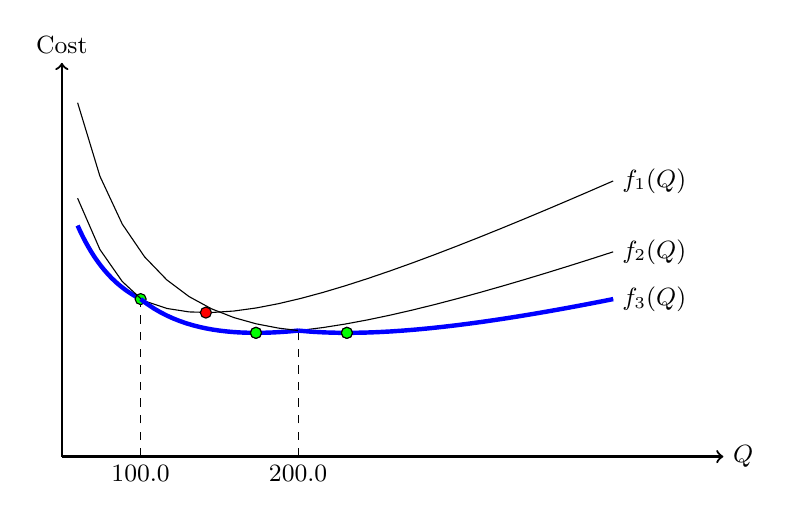
\begin{tikzpicture}[x=0.02cm,y=0.10cm]
\small
\def\c{1} 
\def\K{100} 
\def\h{0.2} 
\def\d{20} 
\def\alpha{0.2}
\def\w{100}
\draw[thick,->] (50,30) -- (470,30) node[right] {$Q$};
\draw[thick,->] (50,30) -- (50,80) node[above] {Cost};
\foreach \n/\a/\b/\c in {1/2000/20/0.1,2/2400/18/0.08,3/3200/18/0.06} {
	\pgfmathsetmacro{\Q}{sqrt(\a)/sqrt(\c)}	
	\pgfmathsetmacro{\f}{\a/\Q+\b+\c*\Q}	
	\pgfmathsetmacro{\s}{(\n-1)*\w}	
	\pgfmathsetmacro{\e}{\n*\w}

	\draw[domain=60:400] plot (\x,{\a/\x+\b+\c*\x}) node[right] {$f_{\n}(Q)$};

	\ifnum\n<3
		\draw[color=blue,ultra thick,domain={max(60,\s}:\e] plot (\x,{\a/\x+\b+\c*\x});
		\draw[dashed] (\e,30) -- (\e,{\a/\e+\b+\c*\e});
		\draw (\e,30) node[below] {$\e$};
	\else
		\draw[color=blue,ultra thick,domain={max(60,\s}:400] plot (\x,{\a/\x+\b+\c*\x});
	\fi

	\draw [fill=red] (\Q,\f) circle (2pt);

	\pgfmathparse{int(\Q-\s)}
	\ifnum \pgfmathresult < 0
		\draw [fill=green] (\s,{\a/\s+\b+\c*\s}) circle (2pt);
	\fi
	\pgfmathparse{int(\Q-\e)}
	\ifnum \pgfmathresult > 0
		\draw [fill=green] (\e,{\a/\e+\b+\c*\e}) circle (2pt);
	\fi
	\pgfmathparse{int((\Q-\e)*(\Q-\s))}
	\ifnum \pgfmathresult < 0
		\draw [fill=green] (\Q,\f) circle (2pt);
	\fi
}
\end{tikzpicture}
\caption{Incremental discounts -- average costs}
\label{fig:avgcost_incremental}
\end{figure}


What we observe here is the following.
\begin{itemize}
\item $f_1(Q)$: This function applies in the $[0,100)$ interval (blue area). It's optimal point is at $141.42$. This point does not fall into function's interval (that's why it is a red dot). Because the function is convex and it's optimal point is to the right of the interval, the minimum point that falls into function's interval is 100 (green dot) which gives a cost of \$50. 
\item $f_2(Q)$: This function applies in the $[100,200)$ interval (blue area). It's optimal point is at $173.21$. This point indeed fall into function's interval (that's why it is a green dot) and it gives a cost of \$45.7. 
\item $f_3(Q)$: This function applies in the $[200,\infty)$ interval (blue area). It's optimal point is at $230.94$. This point indeed fall into function's interval (that's why it is a green dot) and it gives a cost of \$45.7.  
\end{itemize}

Based on these observations, we can conclude that the minimum average cost per unit time we can attain is \$45.7. To achieve that, our order quantity should either be 173.21 units or 230.94 units.
\end{solution}
\end{exercise}


\subsection{To Be Done}
\label{sec:be-done}

\paragraph{Strategic impact of short leadtimes/small inventories,
 what if lead time is a control?}

You run a pharmaceutical company. The medicines you sell need to be
packaged. The price quotation of the company that prints the packages
depends on the order size $Q$.
 \begin{itemize}
 \item If $Q$ covers 2 weeks of demand: price per unit is 1.15 Euro
 \item If $Q$ covers 1 month of demand: price per unit is 1. Euro
 \item If $Q$ covers 2 months of demand: price per unit is 0.95 Euro
 \item If $Q$ covers 3 months of demand: price per unit is 0.9 Euro
 \item If $Q$ covers 6 months of demand: price per unit is 0.85 Euro
 \end{itemize}
The problem is to determine how much to order.

\begin{exercise}
 \begin{itemize}
 \item Include your own storage cost, i.e., packages need to be
   stored as your raw materials inventory.  Suppose the
   inventory cost is $20\%$ per unit per year. Can we now compute the
   inventory cost?  Assume that $D = 12000$ units per year.
 \item Include transportation cost.  Assume that $A = 50$ Euro.
 \end{itemize}
\end{exercise}

\begin{exercise}
Every so often government regulations change. As a result, the entire
stock becomes obsolete. What now?
\begin{solution}
 \begin{itemize}
 \item Use data to make assumptions on the probability that the
   remaining stock will be affected by a regulation change.
 \item Assume that a regulation change occurs, on average, every
   month, and time to implement the change is one month.
 \item If  $Q$ is 2 weeks of demand, then?  there is no problem
 \item If $Q$ is 3 months of demand, then? 
 \end{itemize}
Challenge: Can you compute the optimal order quantity in this situation? 

  \begin{pyconsole}[eoq]
A = 50.
D = 12000
h = 0.2

def C(Q, p): # return average yearly inventory cost
    # p is price per unit, so that
    # p*h is the inventory cost per unit per year
    cost = A*D/Q + h*p*Q/2.
    return cost

def output(Q, p, period):
    print("Yearly inventory costs %s: %3.2f; price of a batch: %3.2f"%(period, C(Q, p), Q*p))

output(D/24, 1.15, "2 weeks")
#Likewise for the other cases.
  \end{pyconsole}

%   \begin{minted}{python}
% Yearly costs 2 weeks: 1257.50; batch price: 575.00
% Yearly costs 1 month: 700.00; batch price: 1000.00
% Yearly costs 2 months: 490.00; batch price: 1900.00
% Yearly costs 3 months: 470.00; batch price: 2700.00
% Yearly costs 6 months: 610.00; batch price: 5100.00
%   \end{minted}

What are the consequences?

 \begin{itemize}
   \item For some customers short lead times are very important. So important
     they are willing to pay significantly more per unit.
   \item For some customers small batch sizes are very important. So
     important they are willing to pay significantly more per unit.
   \item Thus,  it is essential for some/many companies to be
     able to offer short and predictable lead times and produce in
     small batches.
   \item Producing in small batches can be achieved with slack capacity and short setup times and low setup costs.
   \item Short and predictable lead times can be achieved with conwip
     and a order prioritization (priority queues)
 \end{itemize}
\end{solution}
\end{exercise}





\begin{exercise}
EOQ with joint ordering
  \begin{solution}
    TBD
  \end{solution}
\end{exercise}

\begin{exercise}
  Consider the setting of the EOQ model but now with batchsize
  constraints, that is, the order quantity is in multiples of some number $q$, say. Can you make a formula for the cost, and find the minimum?
  \begin{solution}
This is, in fact, really easy. Suppose we order $n$ times the minimal order quantity $q$. Then, for a yearly demand $D$, ordering cost $A$, and inventory cost $h$, we pay per year
\begin{equation*}
  A \frac{D}{nq} + h\frac{nq}2 = A\frac{D/q}n + hq\frac{n}2.
\end{equation*}
But this is precisely the normal EOQ model with demand $D'=D/q$ and inventory cost $h'=hq$. Thus, the optimal number of batches to order is:
\begin{equation*}
  n^2 = \frac{2D'A}{h'} = \frac{2AD/q}{hq} = \frac{2AD}{hq^2}.
\end{equation*}
Hence, the optimal $n$ expressed in the EOQ quantity $Q^*$ is 
\begin{equation*}
  n = \sqrt{\frac{2AD}{h}}\frac1q=\frac{Q^*}q.
\end{equation*}
  \end{solution}
\end{exercise}


\begin{exercise}
EOQ with yield loss
  \begin{solution}
    TBD
  \end{solution}
\end{exercise}

\begin{exercise}
EOQ with lower salvage value
  \begin{solution}
    TBD
  \end{solution}
\end{exercise}


\begin{exercise}
EOQ with constraints on cycle length

EOQ under periodic review rather than continuous review.

Constraints on when to order, order moment.

  \begin{solution}
    TBD
  \end{solution}
\end{exercise}


\begin{exercise}
  EOQ with positive replenishment lead time and variance in the lead
  time.

  \begin{solution}
    TBD

Suddenly we have to deal with safety stock!
  \end{solution}
\end{exercise}

\begin{exercise}
EOQ with variable demand.
  \begin{solution}
    TBD
  \end{solution}
\end{exercise}

\begin{exercise}
Wagner Whitin
  \begin{solution}
    TBD
  \end{solution}
\end{exercise}

\begin{exercise}
Silver meal
  \begin{solution}
    TBD
  \end{solution}
\end{exercise}

\begin{exercise}
Where to put the I/O interface? For what product/item?
  \begin{solution}
    TBD
  \end{solution}
\end{exercise}

\begin{exercise}
  What is the difference between continuous and period review? Why/when to prefer one over the other?
  \begin{solution}
    TBD
  \end{solution}
\end{exercise}

\begin{exercise}
  What is the difference between fixed order and order-up-to policies?
  Why/when to prefer one over the other?
  \begin{solution}
    TBD

Order quantities

  \end{solution}
\end{exercise}

\begin{exercise}
  What  different type of service level can you define?
  Why/when to prefer one over the other?
  \begin{solution}
    TBD

e.g. cycle service level.
  \end{solution}
\end{exercise}

\begin{exercise}
  Why to use safefy stock? What is it? 
  \begin{solution}
    TBD
  \end{solution}
\end{exercise}

\begin{exercise}
  Are lead times typically (approximately) constant ore variable?
  \begin{solution}
    TBD
  \end{solution}
\end{exercise}


\Closesolutionfile{ans}
\opt{solutionfiles}{
\subsection{Solutions}
\input{ans}
}

\clearpage

%%% Local Variables:
%%% mode: latex
%%% TeX-master: "inventory_notes"
%%% End:
